\documentclass[a4paper]{jsarticle}
\pagestyle{empty}  % ページのいる人は消してください
\usepackage{amssymb} 
\usepackage{otf} 
\usepackage[dvipdfmx]{graphicx} % 画像
\usepackage{float}
 \usepackage{bm} % ベクトル
\usepackage{amsmath} 
\usepackage{framed} % 四角で囲む
\usepackage{amsfonts} 
\usepackage{mathabx} 
\usepackage{slashbox}
\usepackage{multicol} % n段組み
\usepackage{algorithm}
\usepackage{algorithmic}
\newcommand{\user}{\textsf{User}}
\newcommand{\server}{\textsf{Server}}
\newcommand{\owner}{\textsf{Owner}}
\newtheorem{Thm}{Theorem}%[section]
\newtheorem{Def}{Definition}%[section]
\newtheorem{Lem}{Lemma}%[section]
\newtheorem{Rem}{Remark}%[section]
%%%%%%% ここからは好きに変えてください %%%%%%%
%\setlength{\textheight}{\paperheight}   
%\setlength{\topmargin}{-18.4mm}     
%\addtolength{\topmargin}{-\headheight} 
%\addtolength{\topmargin}{-\headsep} 
%\addtolength{\textheight}{-14mm}    
%\setlength{\textwidth}{\paperwidth}     
%\setlength{\oddsidemargin}{-19.4mm}  
%\setlength{\evensidemargin}{-19.4mm}  
%\addtolength{\textwidth}{-12mm}     
%%%%%%%%%%%%%%%%%%%%%%%%%%%%%%%%%%%%%
% 文章始まり
\begin{document}


\begin{center}
\LARGE{\textbf{\underline{ペアリングによる内積計算}}}
\end{center}
%%%%%% ここからまとめるときに使う箇所 %%%%%%%%%%%%
% jsreportでまとめるときに\chapter{序論}の下に
% \section{}が来るので独自に議論をまとめて下さい.
\section{Weilペアリング}
有限体$\mathbb{F}_p$上の楕円曲線$E/\mathbb{F}_p$,その上の座標$E(\mathbb{F}_p)$について,$q$等分部分群$E[q]$を次のように定義する.
\begin{align}
E[q]:=\{ \forall P\in E(\mathbb{F}_p):qP=\mathcal{O}\}.
\end{align}
そして,$E[p^e]\simeq \mathbb{Z}/p^e\mathbb{Z}$のとき,この楕円曲線を\textbf{超特異(supersingular)}と呼び,$E[p^e]\simeq \{ \mathcal{O}\}$のとき,\textbf{通常(ordinary)}と呼ぶ.ただし,$\forall e\in\mathbb{N}^+$である.また,$\gcd(\mathsf{ch}(\mathbb{F}_p)\footnote{有限体$\mathbb{F}_p$の標数は,$\underbrace{1+1+\cdots + 1}_{p}= 0$なので$\mathsf{ch}(\mathbb{F}_p) = p$である.}, q)=1$のとき,$E[q]\simeq \mathbb{Z}/q\mathbb{Z}\times \mathbb{Z}/q\mathbb{Z}$である.Weilペアリングでは,$\gcd(\mathsf{ch}(\mathbb{F}_p), q)=1$を満たす素数$q\ (\in \mathbb{P})$における部分群$E[q]\simeq \mathbb{Z}/q\mathbb{Z}\times \mathbb{Z}/q\mathbb{Z}$を採用する.


このとき,ペアリング写像$e_q:G_1\times G_2 \rightarrow G_T$が存在する.つまり,$P\in G_1, Q\in G_2$のとき,$e_q(P,Q)\in G_T$である.ただし,$|G_1| = |G_2| = |G_T| = q$である.

\begin{enumerate}
\item[\textbf{(1)}] \textbf{双線型性(bilinear)}\\
$\forall a,\forall b\in\mathbb{Z}_q$のとき,
\begin{align}
\begin{cases}\vspace{0.05in}
e_q(aP,Q) =e_q(P,aQ)=\left\{ e_q(P,Q) \right\}^a  \pmod{p},\\\vspace{0.05in}
e_q(P,bQ) =e_q(bP,Q)=\left\{ e_q(P,Q) \right\}^b  \pmod{p},\\
e_q(aP,bQ)=\left\{ e_q(P,Q) \right\}^{ab}  \pmod{p}.\\
\end{cases}
\end{align}
\item[\textbf{(2)}] \textbf{同一性(identity)}
\begin{align}
e_q(P,P) = 1\pmod{p}.
\end{align}
\item[\textbf{(3)}] \textbf{非縮退(non degenerate)}\\
$\forall Q\in G_2\ (\ne G_1)$のとき,$e_q(P,Q) = 1$ならば,$P=\mathcal{O}$である.よって,
\begin{align}
e_q(P,\mathcal{O}) = e_q(\mathcal{O}, Q) = 1\pmod{p}.
\end{align}
\item[\textbf{(4)}] \textbf{準同型性(homomorphic)}\\
$\forall P,P'\in G_1, \forall Q,Q'\in G_2$のとき,
\begin{align}
e_q(P+P', Q+Q') &= e_q(P, Q+Q')\cdot e_q(P', Q+Q') \pmod{p}&\notag\\
&=e_q(P+P', Q)\cdot e_q(P+P',Q') \pmod{p}&\\
&=e_q(P, Q) \cdot e_q(P, Q') \cdot e_q(P', Q) \cdot e_q(P', Q') \pmod{p}.&\notag
\end{align}

\item[\textbf{(5)}] \textbf{交代性(alternating)}
\begin{align}
e_q(P, Q) = \left\{ e_q(Q,P)\right\}^{-1}\pmod{p}.
\end{align}
\end{enumerate}
\section{内積の秘匿計算プロトコル}
2つのベクトル\ :\ 
\begin{align}
\begin{cases}
\bm{x}:=[x_1, x_2, \cdots, x_n]\in \mathbb{Z}^n_q \cdots \mathsf{User}\\
\bm{y}:=[y_1, y_2, \cdots, y_n]\in \mathbb{Z}^n_q \ \cdots \mathsf{Owner}
\end{cases}
\end{align}
の内積$\bm{x}\cdot \bm{y} = \sum x_j y_j$をWeilペアリングを用いて秘匿計算する.ただし,$\mathsf{User}$は$\mathsf{Owner}$に対して,または$\mathsf{Owner}$は$\mathsf{User}$に対して,自分のベクトルを公開しない.このような秘匿計算を次のような手順に従って行う.
\begin{figure}[!h]
  \begin{center}
   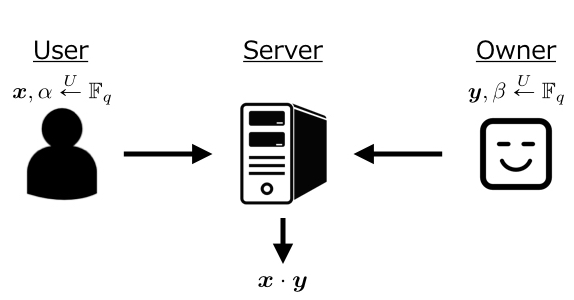
\includegraphics[width=8cm, bb=0 0 575 300]{system.001.jpeg}
  \end{center}
  \caption{System Model}
  \label{SM} %\ref{ラベル}で番号が呼び出せる.
\end{figure}

\begin{enumerate}
\item[\it{(1)}] $\mathsf{User},\mathsf{Server},\mathsf{Owner}$の3者でペアリングに関する情報を共有する.具体的に,有限体$\mathbb{F}_p$,楕円曲線$E/\mathbb{F}_p$,$q$等分部分群$E[q]\simeq \mathbb{Z}/q\mathbb{Z}\times \mathbb{Z}/q\mathbb{Z}$とその位数$q\ (\in \mathbb{P})$,座標$\exists P\in G_1,\exists Q\in G_2$,そしてペアリング写像$e_q:G_1\times G_2 \rightarrow G_T$を3者で共有する.
\item[\it{(2)}] $\mathsf{User}$は,乱数$\alpha \overset{U}{\leftarrow}\mathbb{F}_q $を生成する.ただし,$\mathsf{User}$は$\alpha$を公開しない.
\item[\it{(3)}] $\mathsf{Owner}$は,乱数$\beta \overset{U}{\leftarrow}\mathbb{F}_q $を生成する.ただし,$\mathsf{Owner}$は$\beta$を公開しない.
\item[\it{(4)}]$\mathsf{User}$は,$P$に$x_j$と$\alpha$をスカラー倍した結果\ : $\alpha P,\alpha x_1 P, \alpha x_2 P,\cdots, \alpha x_n P$を$\mathsf{Server}$に送信する.

\item[\it{(5)}]$\mathsf{Owner}$は,$Q$に$y_j$と$\beta$をスカラー倍した結果\ : $\beta Q,\beta y_1 Q, \beta y_2 Q,\cdots, \beta y_n Q$を$\mathsf{Server}$に送信する.
\item[\it{(6)}]$\mathsf{Server}$は,ペアリングの値を計算する.$g:=e_q(P,Q), \ \hat{g}:=e_q(\alpha P,\beta Q) = g^{\alpha\beta}$とすると,
\begin{align}
\begin{cases}
\ e_q(\alpha x_1 P,\beta y_1 Q) = \hat{g}^{x_1y_1} \pmod{p},\\
\ e_q(\alpha x_2 P,\beta y_2 Q) = \hat{g}^{x_2y_2} \pmod{p},\\
\ \ \ \ \ \ \ \ \ \ \ \vdots\\
\ e_q(\alpha  x_n P,\beta y_n Q) = \hat{g}^{x_ny_n}\pmod{p}.
\end{cases}
\end{align}
そして,$\hat{g}^{\bm{x}\cdot\bm{y}} = \hat{g}^{x_1y_1}\times\hat{g}^{x_2y_2}\times \cdots \times \hat{g}^{x_ny_n}$と$\hat{g}$の\textbf{離散対数問題(DLP)}\footnote{離散対数問題は$p$のサイズに依存するが,2012年に923ビットの離散対数問題を計算機で解くことができることをNICTが発表した.ペアリングで用いられる$p$のビット数は,NICTによると224ビットが推奨なので内積を得ることは実現可能である.}を解いて,$\bm{x}\cdot\bm{y}$を得る.
\end{enumerate}

\section{安全性について}
図\ref{SM}のような系の場合,$\mathsf{User}$と$\mathsf{Owner}$は$\mathsf{Server}$に情報を送信するだけなので,相手のベクトルに関する部分情報を一切得ることはできない.しかしながら,$\mathsf{Owner}$は\user と$\mathsf{Server}$との通信を,または$\mathsf{User}$は\owner と$\mathsf{Server}$との通信を盗聴する可能性がある.したがって,Semi-honest-$\mathsf{Server}$,Malicious-$\mathsf{Server}$,Malicious-$\mathsf{Owner}$,Malicious-\user について議論する.



\begin{enumerate}
\item[\textbf{(1)}] Semi-honest-$\mathsf{Server}$\\
 プロトコルに従うが,その途中で得られた情報から積極的に$x_j,y_j$を推測しようとする$\mathsf{Server}$をSemi-honestであると定義する.つまり,安全性の要件として,プロトコル実行中にベクトルの成分の特定に繋がる部分情報を漏らさないことを要求する.

 $\textit{(4)},\textit{(5)}$での安全性の仮定は,\textbf{楕円離散対数問題(ECDLP)}である.つまり,$\alpha x_j P,\ P$や$\beta y_j Q,\ Q$から$\alpha x_j, \beta y_j$を,延いては$\alpha, \beta, x_j, y_j$を求めることはできない.したがって,$\mathsf{Server}$は$\alpha x_j, \beta y_j$を求めることはできない.しかしながら,$\textit{(6)}$で離散対数問題を解くことが可能であると仮定しているので,$\mathsf{Server}$はそれらの積$\alpha x_j\cdot\beta y_j$を求めることができる.ただし,乱数$\alpha, \beta$は公開されていないので,その積から$x_j, y_j$を特定することはできない.

\ \ \ \ 

\item[\textbf{(2)}] Malicious-$\mathsf{Server}$\\
 プロトコルを逸脱し,勝手な振る舞いによって得られた情報から$x_j,y_j$を推測しようとする$\mathsf{Server}$をMaliciousであると定義する.つまり,安全性の要件として,プロトコルなどで得られた情報からベクトルの成分の特定に繋がらないような困難さを要求する.

 まず$\mathsf{Server}$は,楕円離散対数問題をペアリングによって離散対数問題に帰着させることによって,$\alpha,\beta$を特定しようとする.\begin{align}
\begin{cases}
\ e_q(\alpha P,Q) = g^{\alpha} \pmod{p},\\
\ e_q(P,\beta Q) = g^{\beta} \pmod{p}.
\end{cases}
\end{align}
仮定より$(g^\alpha, g, p),(g^\beta, g, p)$の離散対数問題を解くことが可能なので,乱数$\alpha,\beta$を求めることができる.そして,次のようにペアリングの値を計算する.
\begin{align}
\begin{cases}
\ e_q(\alpha x_j P,Q) = g^{\alpha x_j} \pmod{p},\\
\ e_q(P,\beta y_j Q) = g^{\beta y_j} \pmod{p}.
\end{cases}
\end{align}
同様に,$g^{\alpha x_j},g^{\beta y_j}$から離散対数問題を解き,$\alpha x_j,\beta y_j$を得る.最後にそれらの値と$\alpha, \beta$から$\mathsf{Server}$は$x_j,y_j$を求めることができる.

\ \ \ \ \ 

\item[\textbf{(3)}] Malicious-$\mathsf{Owner}$/ Malicious-$\mathsf{User}$\ \\
 通信を盗聴することによって,$x_j$および$y_j$を推測しようとする$\mathsf{Server}$または\user をMaliciousであると定義する.つまり,安全性の要件として,盗聴した情報からベクトルの成分の特定に繋がらないような困難さを要求する.前述のとおり,まず乱数を特定する必要がある.
\begin{align}
\begin{cases}
\ e_q(\alpha P,Q) = g^{\alpha} \pmod{p},\\
\ e_q(P,\beta Q) = g^{\beta} \pmod{p}.
\end{cases}
\end{align}
$(g^\alpha, g, p),(g^\beta, g, p)$の離散対数問題を解くことで容易に乱数$\alpha,\beta$を求めることができる.そして,次のようにペアリングの値を計算する.
\begin{align}
\begin{cases}
\ e_q(\alpha x_j P,Q) = g^{\alpha x_j} \pmod{p},\\
\ e_q(P,\beta y_j Q) = g^{\beta y_j} \pmod{p}.
\end{cases}
\end{align}
同様に,$g^{\alpha x_j},g^{\beta y_j}$から離散対数問題を解き,$\alpha x_j,\beta y_j$を得る.最後にそれらの値と$\alpha, \beta$から$x_j,y_j$を求めることができてしまう.そこで,SSLなどのセキュア通信によって安全性を確保する.


\end{enumerate}

\section{効率性について}
通信量と計算量は,それぞれ次の表\ref{Com2},\ref{Com1}のとおりである.


\begin{table}[htb]
\begin{center}
  \begin{tabular}{|c|c|c|c|} \hline
      \backslashbox{}{}   & $\ \mathsf{User}\ $ & $\mathsf{Server}$ & $\mathsf{Owner}$ \\ \hline 
\it{(4)}& $\mathcal{O}(n)$ & -- & -- \\ \hline 
\it{(5)}& -- & -- & $\mathcal{O}(n)$ \\ \hline 
  \end{tabular}
  \caption{Communication cost of $\mathsf{User}, \mathsf{Server}$ and $\mathsf{Owner}$ }
  \label{Com2} %\ref{ラベル}で番号が呼び出せる.
\end{center}
%\end{table}

\ \ \ 

%\begin{table}[htb]
\begin{center}
  \begin{tabular}{|c|c|c|c|} \hline
      \backslashbox{}{}   & $\ \mathsf{User}\ $ & $\mathsf{Server}$ & $\mathsf{Owner}$ \\ \hline 
\it{(4)}& $\mathcal{O}(n)$ & -- & -- \\ \hline 
\it{(5)}& -- & -- & $\mathcal{O}(n)$ \\ \hline 
\it{(6)}& -- & $\mathcal{O}(n)$ & -- \\ \hline 
  \end{tabular}
  \caption{Computation cost of $\mathsf{User}, \mathsf{Server}$ and $\mathsf{Owner}$ }
  \label{Com1} %\ref{ラベル}で番号が呼び出せる.
\end{center}
\end{table}

\newpage
\begin{center}
\LARGE{\textbf{\underline{ペアリングと述語暗号}}}
\end{center}
\setcounter{figure}{0}
\setcounter{table}{0}
\setcounter{equation}{0}
\setcounter{section}{0}
\section{正準的な双対直交基底}
$n$次元のベクトル空間$V$の正準基底$\mathbb{A}$と相対する$n$次元のベクトル空間$V^*$の正準基底$\mathbb{A}^*$を次のように定義する.
\begin{align}
\mathbb{A} = \{ \bm{a}_1, \bm{a}_2, \cdots, \bm{a}_n \},\ \ 
\mathbb{A}^* = \{ \bm{a}^*_1, \bm{a}^*_2, \cdots, \bm{a}^*_n \}.
\end{align}
そして,$\forall a_i\in\mathbb{F}_q, \forall a^*_i\in\mathbb{F}_q$のとき,
\begin{align}
\begin{cases}
\ \bm{a}_1 = [a_1,0,0,\cdots,0],\\
\ \bm{a}_2 = [0,a_2,0,\cdots,0],\\
\ \ \ \ \ \ \vdots\\
\ \bm{a}_n = [0,0,0,\cdots,a_n],
\end{cases}\ \ 
\begin{cases}
\ \bm{a}^*_1 = [a^*_1,0,0,\cdots,0],\\
\ \bm{a}^*_2 = [0,a^*_2,0,\cdots,0],\\
\ \ \ \ \ \ \vdots\\
\ \bm{a}^*_n = [0,0,0,\cdots,a^*_n].
\end{cases}
\end{align}
このとき,双対直交基底なので次のような関係を満たす.
\begin{align}
\bm{a}_i\cdot \bm{a}^*_j = \delta_{ij}\pmod{q}.
\end{align}
成分$a_i$と$a_i^*$は,次のように選択する.
\begin{align}
a_i\overset{U}{\leftarrow} \mathbb{F}_q,\ \  a_i^*\leftarrow a_i^{-1}\pmod{q}
\end{align}


2つのベクトル$\bm{x},\bm{y}$を次のように定義する.
\begin{align}
\begin{cases}
\bm{x} := [x_1, x_2,\cdots,x_n]\in \mathbb{Z}_q^n\\
\bm{y} := [y_1, y_2,\cdots, y_n]\in \mathbb{Z}_q^n
\end{cases}
\end{align}
内積$\bm{x}\cdot\bm{y}$を次のように秘匿計算するため,$x_c,y_c$を次のように定義する.
\begin{align}
x_c := \displaystyle\sum_{j=1}^n x_j\bm{a}_j \left(= \sum_{j=1}^n x_ja_j\right),\ \ 
y_c := \displaystyle\sum_{j=1}^n y_j\bm{a}^*_j \left(= \sum_{j=1}^n y_ja^*_j\right).
\end{align}

$g:=e_q(P,Q)\ (\ne 0)$とするとき,$\mathbb{A}, \mathbb{A}^*$は次のような関係を満たす.
\begin{align}
e_q(\bm{a}_iP, \bm{a}^*_jQ) = g^{\sum\bm{a}_i\cdot\bm{a}^*_j} = g^{\delta_{ij}}\pmod{p}.
\end{align}


$n$次元ベクトル空間$V,V^*$におけるペアリング演算$e_q$は,
\begin{align}
e_q(x_cP, y_cQ) := \prod_{j=1}^n e_q(x_j\bm{a}_jP, y_j\bm{a}^*_jQ) = e_q(P, Q)^{\sum x_jy_j\bm{a}_j\cdot\bm{a}^*_j}=g^{\bm{x}\cdot\bm{y}}\pmod{p}.
\end{align}

\section{双対直交基底の一般線形変換}
ユニタリ行列$X:=(\chi_{ij})\overset{U}{\leftarrow} GL(n, \mathbb{F}_p)$を用いて,正準基底$\mathbb{A},\mathbb{A}^*$を$\mathbb{B},\mathbb{B}^*$に変換する.ユニタリ行列なので,$U=(U^T)^{-1}$を満たす.したがって,
\begin{align}
\bm{b}_i = \sum_{j=1}^n \chi_{ij}\bm{a}_j,\ \ \bm{b}_j^* = \sum_{i=1}^n (\chi_{ji})^{-1}\bm{a}_i^*.
\end{align}
そして,$X^TX=E$なので$\bm{b}_i\cdot\bm{b}^*_j = \bm{a}_i\cdot\bm{a}_j^*=\delta_{ij}$である.したがって,$\mathbb{B},\mathbb{B}^*$は次のような関係を満たす.
\begin{align}
e_q(\bm{b}_i, \bm{b}^*_j) = g^{\delta_{ij}}\pmod{p}.
\end{align}



\section{1階層内積述語暗号}
$n+3$次元のペアリングベクトル空間$(p,V,V^*, G_T, \bm{B},\bm{B}^*)$を考える.
\begin{align}
\begin{cases}
\ \mathbb{B} = \{ \bm{b}_1, \bm{b}_2, \cdots, \bm{b}_n, \bm{b}_{n+1},\bm{b}_{n+2},\bm{b}_{n+3}\},\\
\ \mathbb{B}^* = \{ \bm{b}^*_1, \bm{b}^*_2, \cdots, \bm{b}^*_n, \bm{b}^*_{n+1},\bm{b}^*_{n+2},\bm{b}^*_{n+3} \},\\
\ \hat{\mathbb{B}} = \{ \bm{b}_1, \bm{b}_2, \cdots, \bm{b}_n, \bm{d}_{n+1},\bm{b}_{n+3} \}.
\end{cases}
\end{align}

\begin{itemize}
\item[\textbf{(1)}] \textbf{Key Generation}\\
 $\bm{x} = [x_1,x_2,\cdots,x_n]\ \in \mathbb{F}_q$を\textbf{属性ベクトル},$\bm{v} = [v_1, v_2, \cdots, v_n]\ \in \mathbb{F}_q$を\textbf{述語ベクトル}と呼ぶ.ただし,$\bm{x}\cdot \bm{v} = 0$を満たすように設定する.そして,$\sigma, \eta\overset{U}{\leftarrow}\mathbb{F}_q$とするとき,
\begin{align}
k^* := \sigma(v_1\bm{b}^*_1 + \cdots + v_n\bm{b}^*_n) + \eta\bm{b}^*_{n+1} + (1-\eta)\bm{b}^*_{n+2}.
\end{align}
このとき,$\mathbb{B}^*, k^*$を秘密鍵$sk$,$\hat{\mathbb{B}}$を公開鍵$pk$とする.

\item[\textbf{(2)}] \textbf{Encryption}\\
$\delta_1, \delta_2, \zeta\overset{U}{\leftarrow}\mathbb{F}_q,\ \bm{d}_{n+1}:=\bm{b}_{n+1} + \bm{b}_{n+2}$
のとき,次のように平文$m\ (\in\mathbb{Z}_p)$を暗号化する.
\begin{align}
\begin{cases}
c_1 = \delta_1 (x_1\bm{b}_1 + \cdots + x_n\bm{b}_n)+\zeta \bm{d}_{n+1} + \delta_2 \bm{b}_{n+3},\\
c_2 = g^\zeta\cdot m\pmod{p}.
\end{cases}
\end{align}
\item[\textbf{(3)}] \textbf{Decryption}
\begin{align}
e_q(c_1,k^*) &= \prod_{i=1}^n e_q(\delta_1 x_i\bm{b}_i, \sigma v_i\bm{b}^*_i)\cdot e_q(\zeta\bm{b}_{n+1},\eta\bm{b}^*_{n+1})\cdot e_q(\zeta\bm{b}_{n+2},(1-\eta)\bm{b}^*_{n+2})&\\
&=g^{\delta_1\sigma\sum x_iv_i}\cdot g^{\zeta\eta}\cdot g^{\zeta(1-\eta)}=g^\zeta\pmod{p}.&
\end{align}
よって,次のように復号する\footnote{秘密鍵を持っていても属性ベクトル$\bm{x}$が$\bm{x}\cdot\bm{v} = 0$を満たさない場合,復号することができない.}.
\begin{align}
\dfrac{c_2}{e_q(c_1,k^*)} = m\pmod{p}.
\end{align}
\end{itemize}

\newpage
\begin{center}
\LARGE{\textbf{\underline{類似検索可能暗号の実装評価}}}
\end{center}
\setcounter{figure}{0}
\setcounter{table}{0}
\setcounter{equation}{0}
\setcounter{section}{0}
\section{重み付きEuclid距離の秘匿計算プロトコル}
2つのベクトル\ :\ 
\begin{align}
\begin{cases}
\bm{x}:=[x_1, x_2, \cdots, x_n]\in \mathbb{Z}^n_q \cdots \mathsf{User}\\
\bm{y}:=[y_1, y_2, \cdots, y_n]\in \mathbb{Z}^n_q \ \cdots \mathsf{Owner}
\end{cases}
\end{align}
の重み付きEuclid距離$l_{xy}=\sum w_j|x^2_j - y^2_j|$の2乗$l_{xy}^2$をWeilペアリングを用いて秘匿計算する.ただし,$\mathsf{User}$は$\mathsf{Owner}$に対して,または$\mathsf{Owner}$は$\mathsf{User}$に対して,自分のベクトルを公開しない.このような秘匿計算を次のような手順に従って行う.
\begin{figure}[!h]
  \begin{center}
   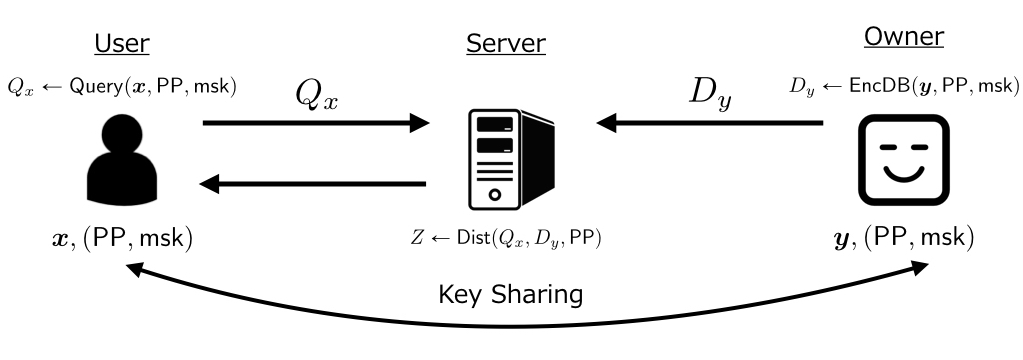
\includegraphics[width=10cm, bb=0 0 1018 360]{system.002.jpeg}
  \end{center}
  \caption{System Model}
  \label{SM1} %\ref{ラベル}で番号が呼び出せる.
\end{figure}


\begin{enumerate}
\item[\it{(1)}] \owner は,$n$個の重み$w_j\ (\in \mathbb{Z}_q)$を設定し公開する.
\item[\it{(2)}] \user は,$\bm{x}$を次のように符号化し$\bm{x}''$を得る.ただし,$|\bm{x}''| = n + 4$である.
\begin{align}
\begin{cases}
\ x'_1 = \sum w_jx_j^2,\ \ x'_2\leftarrow 1, \\
\ x'_j= -2w_{j-2}x_{j-2}\ \ (j = 3,4,\cdots,n+2).
\end{cases}
\end{align}
さらに,$(0,1)$を追加する.
\begin{align}
\bm{x}'' = (0,1,x'_1,\cdots, x'_{n+2}).
\end{align}
\item[\it{(3)}] \owner は,$\bm{y}$を次のように符号化して$\bm{y}''$を得る.ただし,$|\bm{y}''| = n + 4$である.
\begin{align}
\begin{cases}
\ y'_1 = 1 ,\ \ y'_2\leftarrow \sum w_jy^2_j, \\
\ y'_j= y_{j-2}\ \ (j = 3,4,\cdots,n+2).
\end{cases}
\end{align}
さらに,$(1,0)$を追加する.
\begin{align}
\bm{y}'' = (1,0,y'_1,\cdots, y'_{n+2}).
\end{align}
\item[\it{(4)}] \owner はマスター鍵$\mathsf{msk}$を生成し,\user と共有する.具体的に,2つの双対直交基底$(\mathbb{B},\mathbb{B}^*),\ (\mathbb{D},\mathbb{D}^*)$である.ただし,$|\mathbb{B}| = |\mathbb{B}^*| = 2(n+4),\ \ |\mathbb{D}| = |\mathbb{D}^*| = 2$である.
\begin{align}
\begin{cases}
\ \mathbb{B} = [\bm{b}_1, \cdots, \bm{b}_{2n+8}],\ 
\mathbb{B}^* = [\bm{b}_1^*, \cdots, \bm{b}^*_{2n+8}],\\ 
\ \mathbb{D}=[\bm{d}_1,\bm{d}_2],\ 
\mathbb{D}^*=[\bm{d}_1^*,\bm{d}^*_2].
\end{cases}
\end{align}
双対直交基底なので,$\bm{b}_i\cdot \bm{b}_j^* = \delta_{ij},\ \bm{d}_i\cdot \bm{d}_j^* = \delta_{ij}$を満たす.したがって,マスター鍵は,
\begin{align}
\mathsf{msk} = [\mathbb{B},\mathbb{B}^*,\mathbb{D},\mathbb{D}^*].
\end{align}
\item[\it{(5)}] $\mathsf{User},\mathsf{Server},\mathsf{Owner}$の3者でペアリングに関する公開パラメタ$\mathsf{PP}$を共有する.具体的に,有限体$\mathbb{F}_p$,楕円曲線$E/\mathbb{F}_p$,$q$等分部分群$E[q]\simeq \mathbb{Z}/q\mathbb{Z}\times \mathbb{Z}/q\mathbb{Z}$とその位数$q\ (\in \mathbb{P})$,座標$\exists P\in G_1,\exists Q\in G_2$,そしてペアリング写像$e_q:G_1\times G_2 \rightarrow G_T$を3者で共有する.したがって,公開パラメタは,
\begin{align}
\mathsf{PP} = [G_1, G_2, G_T, P, Q, p,q].
\end{align}
\item[\it{(6)}] \user は,検索クエリ$Q_x=(Q_x^{(1)}, Q_x^{(2)})$をつくり\server に送信する.$\beta, \beta^* \overset{U}{\leftarrow} \mathbb{F}_q $を用いて,
\begin{align}
\displaystyle
\begin{cases}
\ Q_x^{(1)} = \left( \beta\sum_{j = 1}^{n+4} x''_j \bm{b}_j + \beta^*\sum_{j = 1}^{n+4} x''_j \bm{b}_{n+4+j}\right) Q,\\
\ Q_x^{(2)} = \left( \beta \bm{d}_1  + \beta^* \bm{d}_2 \right) Q.
\end{cases}
\end{align}
\item[\it{(7)}] \owner は,参照データベース$D_y=(D_y^{(1)}, D_y^{(2)})$をつくり\server に送信する.$\alpha, \alpha^* \overset{U}{\leftarrow} \mathbb{F}_q $を用いて,
\begin{align}
\displaystyle
\begin{cases}
\ D_y^{(1)} = \left( \alpha\sum_{j = 1}^{n+4} y''_j \bm{b}^*_j + \alpha^*\sum_{j = 1}^{n+4} y''_j \bm{b}^*_{n+4+j}\right) P,\\
\ D_y^{(2)} = \left( \alpha \bm{d}^*_1  + \alpha^* \bm{d}^*_2 \right) P.
\end{cases}
\end{align}
\item[\it{(8)}] \server は,あらかじめ$M$個の参照データベース$D_y$を\owner から得ている仮定とする.そして,\user から検索クエリ$Q_x$を受け取り,次のようなペアリングの値を計算する.ここで,$g:=e_q(P,Q)\ (\ne 0)$とすると,
\begin{align}
\begin{cases}
\ D_1 = e_q(D_y^{(1)},Q_x^{(1)}) = g^{(\alpha\beta + \alpha^*\beta^*)\sum x''_jy''_j}\pmod{p},\\
\ D_2 = e_q(D_y^{(2)},Q_x^{(2)}) = g^{\alpha\beta + \alpha^*\beta^*}\pmod{p}.
\end{cases}
\end{align}

\item[\it{(9)}] \server は,$(D_1, D_2, p)$の離散対数問題を解き,$\sum x''_j y''_j = l_{xy}$を得る.そして,\server は,$l_{xy}$からある基準によって何かを判断し,それに相当する何らかの情報を\user に送信する.
\end{enumerate}






\section{実装上の注意点}
\begin{enumerate}
\item[\it{(1)}] 簡単のため$w_j=1$とする.
\item[\it{(4)}] 双対直交基底$(\mathbb{B},\mathbb{B}^*)$は,正準的な双対直交基底$(\mathbb{A},\mathbb{A}^*)$をユニタリ行列$X\overset{U}{\leftarrow}GL(n,q)$によって線形変換することによってつくることが可能である.
\begin{enumerate}
\item[\it{(4-1)}] 正準的な直交基底の成分は,$\forall a_i\in\mathbb{F}_q, \forall a^*_i\in\mathbb{F}_q$のとき,
\begin{align}
\begin{cases}
\ \bm{a}_1 = [a_1,0,0,\cdots,0],\\
\ \bm{a}_2 = [0,a_2,0,\cdots,0],\\
\ \ \ \ \ \ \vdots\\
\ \bm{a}_n = [0,0,0,\cdots,a_n],
\end{cases}\ \ 
\begin{cases}
\ \bm{a}^*_1 = [a^{-1}_1,0,0,\cdots,0],\\
\ \bm{a}^*_2 = [0,a^{-1}_2,0,\cdots,0],\\
\ \ \ \ \ \ \vdots\\
\ \bm{a}^*_n = [0,0,0,\cdots,a^{-1}_n].
\end{cases}
\end{align}
このとき,
\begin{align}
\bm{a}_i\cdot \bm{a}^*_j = \delta_{ij}\pmod{q}.
\end{align}


\item[\it{(4-2)}] $r_j \overset{U}{\leftarrow}\mathbb{F}_q$を用いて$(\mathbb{A},\mathbb{A}^*)$から$(\mathbb{B},\mathbb{B}^*)$に線形変換する.
\begin{align}
\begin{cases}
\ \bm{b}_1 = [a_1^{r_1},0,0,\cdots,0],\\
\ \bm{b}_2 = [0,a_2^{r_2},0,\cdots,0],\\
\ \ \ \ \ \ \vdots\\
\ \bm{b}_n = [0,0,0,\cdots,a_n^{r_n}],
\end{cases}\ \ 
\begin{cases}
\ \bm{b}^*_1 = [a^{-r_1}_1,0,0,\cdots,0],\\
\ \bm{b}^*_2 = [0,a^{-r_2}_2,0,\cdots,0],\\
\ \ \ \ \ \ \vdots\\
\ \bm{b}^*_n = [0,0,0,\cdots,a^{-r_n}_n].
\end{cases}
\end{align}

$\mathbb{D},\mathbb{D}^*$も同様に,$\bar{a}_j\overset{U}{\leftarrow}\mathbb{F}_q,\ \bar{r}_j \overset{U}{\leftarrow}\mathbb{F}_q$において,
\begin{align}
\bm{d}_1 = [\bar{a}^{\bar{r}_1}_1,0],\ \ \bm{d}_2 = [0,\bar{a}^{\bar{r}_2}_2],\ \bm{d}^*_1 = [(\bar{a}^{\bar{r}_1}_1)^{-1},0],\ \ \bm{d}^*_2 = [0,(\bar{a}^{\bar{r}_2}_2)^{-1}].
\end{align}
\end{enumerate}
\item[\it{(6)}] \it{(4)}に従うと,
\begin{align}
\displaystyle
\ Q_x^{(1)} = \begin{bmatrix} 
\beta x''_1 b_1 Q, & \beta^* x''_1 b_{n+5} Q, \vspace{0.02in}\\
\beta x''_2 b_2 Q, & \beta^* x''_2 b_{n+6} Q, \\
\vdots & \vdots \vspace{0.02in}\\
\beta x''_{n+4} b_{n+4} Q, & \beta^* x''_{n+4} b_{2n+8} Q, \\
\end{bmatrix} 
,\ Q_x^{(2)} = [\beta d_1 Q ,\beta^* d_2 Q].
\end{align}
\item[\it{(7)}] \it{(4)}に従うと,
\begin{align}
\displaystyle
\ D_y^{(1)} = \begin{bmatrix} 
\alpha y''_1 b^*_1 P, & \alpha^* y''_1 b^*_{n+5} P, \vspace{0.02in}\\
\alpha y''_2 b^*_2 P, & \alpha^* y''_2 b^*_{n+6} P, \\
\vdots & \vdots \vspace{0.02in}\\
\alpha y''_{n+4} b^*_{n+4} P, & \alpha^* y''_{n+4} b^*_{2n+8} P, \\
\end{bmatrix} 
,\ D_y^{(2)} = [\alpha d_1^* P ,\alpha^* d_2^* P].
\end{align}

\item[\it{(8)}] $g:=e_q(P,Q)\ (\ne 0)$とするとき,ペアリングは次のように計算する.
\begin{align}
e_q(D_y^{(1)}, Q_x^{(1)}) &= \prod_{j = 1}^{n+4} e_q(\alpha y''_j b_j^* P, \beta x''_j b_j Q)\times \prod_{j = 1}^{n+4} e_q(\alpha^* y''_j b_{j+n+4}^* P, \beta^* x''_j b_{j+n+4} Q) \notag\\&\ = g^{\alpha\beta\sum x_j''y_j''}\times g^{\alpha^*\beta^*\sum x_j''y_j''} =g^{(\alpha\beta + \alpha^*\beta^*)\sum  x_j''y_j''}\pmod{p},\\
e_q(D_y^{(2)}, Q_x^{(2)}) &=e_q(\alpha d_1^* P, \beta d_1 Q)\times e_q(\alpha^* d_2^* P, \beta^* d_2 Q) = g^{\alpha\beta + \alpha^*\beta^*}\pmod{p}.
\end{align}
\end{enumerate}
\section{安全性について}


図\ref{SM1}のような系の場合,$\mathsf{User}$と$\mathsf{Owner}$は$\mathsf{Server}$に情報を送信し,\server も\user に情報を返信する.したがって,\owner は,相手のベクトルに関する部分情報を一切得ることはできない.しかしながら,$\mathsf{Owner}$は\user と$\mathsf{Server}$との通信を盗聴する可能性がある.ただし,\owner が\server に参照データベースを置いてからサービスが開始するため,\user が\owner と\server の通信を盗聴することを想定しない.したがって,Semi-honest-$\mathsf{Server}$,Malicious-$\mathsf{Server}$,Malicious-$\mathsf{Owner}$ について議論する.




\begin{enumerate}
\item[\textbf{(1)}] Semi-honest-$\mathsf{Server}$\\
 プロトコルに従うが,その途中で得られた情報から積極的に$x''_j,y''_j$を推測しようとする$\mathsf{Server}$をSemi-honestであると定義する.つまり,安全性の要件として,プロトコル実行中にベクトルの成分の特定に繋がる部分情報を漏らさないことを要求する.

 $\textit{(6)},\textit{(7)}$での安全性の仮定は,楕円離散対数問題である.$\beta x''_j b_j P$や$\alpha y''_j b_j^* Q$から$\beta x''_j b_j, \alpha y''_j b_j^* y_j$を,延いては$\alpha, \beta, x''_j, y''_j$を求めることはできない.したがって,$\mathsf{Server}$は$\beta x''_j b_j, \alpha y''_j b_j^*$を求めることはできない.しかしながら,離散対数問題を解くことが可能であると仮定しているので,$\mathsf{Server}$はそれらの積を求めることができる.ただし,乱数$\alpha, \beta$は公開されていないので,その積から$x''_j, y''_j$を特定することはできない.

\ \ \ \ 

\item[\textbf{(2)}] Malicious-$\mathsf{Server}$\\
 プロトコルを逸脱し,勝手な振る舞いによって得られた情報から$x_j,y_j$を推測しようとする$\mathsf{Server}$をMaliciousであると定義する.つまり,安全性の要件として,プロトコルなどで得られた情報からベクトルの成分の特定に繋がらないような困難さを要求する.

 まず,$\mathsf{Server}$は,ペアリングによって楕円離散対数問題を離散対数問題に還元することで係数を求めることが可能である.
\begin{align}
\begin{cases}
\ \alpha y''_jb_j^*,\ \alpha^* y''_j b^*_{j+5},\ \alpha d_1^*,\ \alpha^* d_2^*,\\
\ \beta x''_jb_j,\ \beta^* x''_j b^*_{j+5},\ \beta d_1,\ \beta^* d_2,\\
\ \alpha\beta x_j'' y_j'',\ \alpha^*\beta^* x_j'' y_j''.
\end{cases}
\end{align}
しかし,マスター鍵\ :\ $(\mathbb{B},\mathbb{B}^*,\mathbb{D},\mathbb{D}^*)$と乱数\ :\ $(\alpha,\alpha^*,\beta,\beta^*)$を同時に特定することはできないので,Maliciousといへどもベクトルの成分の特定は困難であるといえる.

 次に,検索クエリや参照データベースの識別可能性について議論するために,次のようなゲームを考える.図\ref{Game1}の\textsf{Challenger}は,\owner と\user に相当し,\textsf{Adversary}はMalicious-\server に相当する.

\begin{figure}[!h]
  \begin{center}
   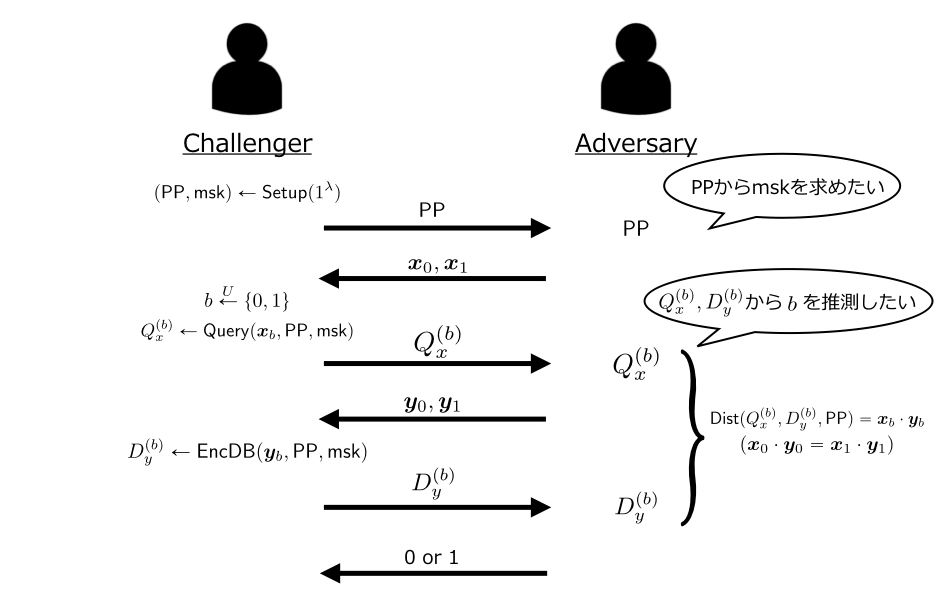
\includegraphics[width=13cm, bb=0 0 809 605]{system.003.jpeg}
  \end{center}
  \caption{Security Game}
  \label{Game1} %\ref{ラベル}で番号が呼び出せる.
\end{figure}

 検索クエリ$Q_x$や参照データベース$D_y$は,乱数$\alpha, \alpha^*,\beta,\beta^*$を用いて生成する.これらの乱数は$Q_x,D_y$を生成する度に生成するため,\textsf{Adversary}はこの乱数を$Q_x,D_y$から特定することができなければ,$Q_x,D_y$を多く集めても識別することは不可能である.しかし,前述のとおり\textsf{Server}は,乱数を特定することはできない.また,双対直交基底も乱数を用いて生成しているので,\owner から$\mathsf{msk}$についての情報が漏れない限り,\textsf{Server}は\textsf{msk}を特定することはできない.したがって,$Q_x,D_y$からベクトルの成分を特定するための部分情報は一切漏れない.

\ \ \ \ 



\item[\textbf{(3)}] Malicious-$\mathsf{Owner}$\\
 \user と\server の通信を盗聴することによって,$x_j$を推測しようとする\owner をMaliciousであると定義する.つまり,安全性の要件として,盗聴した情報からベクトルの成分の特定に繋がらないような困難さを要求する.

 まず,\owner は次のようにペアリングにより還元して乱数を求める.
\begin{align}
\begin{cases}
\ e_q(d_1^*P,\beta d_1 Q) = g^{\beta}\pmod{p},\\
\ e_q(d_2 P,\beta^* d_2 Q) = g^{\beta^*}\pmod{p}.
\end{cases}
\end{align}
そして\owner は,$\alpha\beta x''_j y''_j$から$\alpha, \beta, y_j$を用いて$x_j$を特定する.このように\owner は盗聴することで簡単に\user のベクトルの成分を求めることができてしまう.そこで,SSLなどのセキュア通信によって安全性を確保する.
\end{enumerate}





\vspace{-0.1in}
\section{効率性について}
通信量と計算量は,それぞれ次の表\ref{Com4},\ref{Com3}のとおりである.
\begin{table}[htb]
\begin{center}
  \begin{tabular}{|c|c|c|c|} \hline
      \backslashbox{}{}   & $\ \mathsf{User}\ $ & $\mathsf{Server}$ & $\mathsf{Owner}$ \\ \hline 
\it{(6)}& $\mathcal{O}(n)$ & -- & -- \\ \hline 
\it{(7)}& -- & -- & $\mathcal{O}(Mn)$ \\ \hline 
  \end{tabular}
  \caption{Computation cost of $\mathsf{User}, \mathsf{Server}$ and $\mathsf{Owner}$ }
  \label{Com4} %\ref{ラベル}で番号が呼び出せる.
\end{center}
%\end{table}

 \ \ \ \ 

%\begin{table}[htb]
\begin{center}
  \begin{tabular}{|c|c|c|c|} \hline
      \backslashbox{}{}   & $\ \mathsf{User}\ $ & $\mathsf{Server}$ & $\mathsf{Owner}$ \\ \hline 
\it{(2)}& $\mathcal{O}(n)$ & -- & -- \\ \hline 
\it{(3)}& -- & -- & $\mathcal{O}(n)$ \\ \hline 
\it{(6)}& $\mathcal{O}(n)$ & -- & -- \\ \hline 
\it{(7)}& -- & -- & $\mathcal{O}(n)$ \\ \hline 
\it{(8)}& -- & $\mathcal{O}(Mn)$ & -- \\ \hline 
\it{(9)}& -- & -- & $\mathcal{O}(M)$ \\ \hline
  \end{tabular}
  \caption{Communication cost of $\mathsf{User}, \mathsf{Server}$ and $\mathsf{Owner}$ }
  \label{Com3} %\ref{ラベル}で番号が呼び出せる.
\end{center}
\end{table}






\end{document}
%%%%%%%%%%%%%%%%%%%%%%%%%%%%%%%%%%%%%%%%%
% 文章終わり
%%% 図の挿入のテンプレ
\begin{figure}[!h]
  \begin{center}
   \includegraphics[width=10cm, bb=0 0 100 100]{photo_4.png}
  \end{center}
  \caption{キャプション}
  \label{ラベル} %\ref{ラベル}で番号が呼び出せる.
\end{figure}
図\ref{ラベル}に関する説明.


\begin{algorithm}                      
\caption{Calculate $y = x^n$}         
\label{alg1}                          
\begin{algorithmic}                  
\REQUIRE $n \geq 0 \vee x \neq 0$
\ENSURE $y = x^n$
\STATE $y \Leftarrow 1$
\IF{$n < 0$}
\STATE $X \Leftarrow 1 / x$
\STATE $N \Leftarrow -n$
\ELSE
\STATE $X \Leftarrow x$
\STATE $N \Leftarrow n$
\ENDIF
\WHILE{$N \neq 0$}
\IF{$N$ is even}
\STATE $X \Leftarrow X \times X$
\STATE $N \Leftarrow N / 2$
\ELSE[$N$ is odd]
\STATE $y \Leftarrow y \times X$
\STATE $N \Leftarrow N - 1$
\ENDIF
\ENDWHILE
\end{algorithmic}
\end{algorithm}


その確率は,例えば正解が$\alpha = \prod^{\hat{r}} \hat{s}_j^{\hat{d}_j}\ (\hat{s}_j\in \mathbb{P})$である場合,次のように表すことができる.
\begin{align}
\mathsf{Prob}[\alpha = \alpha'] < \dfrac{2}{\displaystyle\prod^{\hat{r}} \hat{d}_j^{\hat{r}}}.
\end{align}
通常,$\mathsf{Prob}[\alpha = \alpha', \beta = \beta']<\mathsf{Prob}[\alpha = \alpha']$なので,十分に安全性を確保できないと判断する場合は,SSLなどのセキュア通信によって安全性を確保する必要がある.








このとき,仮定より$\hat{g}$から$\alpha\beta$を求めることは簡単である.そこで,$\alpha\beta$を分解して$\alpha,\beta$にすることが難しいように乱数を選ぶようにしなければいけない.しかしながら,$q$のサイズでは$p$に\textbf{Sophie Germain 素数}\footnote{$p = 2 q + 1$を満たす素数$p,q$を\textbf{安全素数(safe prime)}と呼ぶ.安全素数をフランスの物理学者Sophie Germain(1776 - 1831)の名を借りて\textbf{Sophie Germain prime}と呼ぶこともある.}を用いても\textbf{素因数分解問題(IFP)}は解くことが可能であるため,$\alpha,\beta$を大きな素数で守ることはできない.したがって,多くの素因数から構成される乱数を生成する必要がある.

 $\alpha\beta =  \prod^r s_j^{d_j}\ (s_j\in \mathbb{P})$のように素因数分解されるとき,$\alpha,\beta$の候補は約数の個数$\prod^r (1 + d_j)$の半分である.したがって,$\mathsf{Server}$が$\alpha,\beta$の特定するために必要な計算量は$\mathcal{O}\left(\prod d_j^r\right)$であり,特定することができる確率$\mathsf{Prob}[\alpha = \alpha', \beta = \beta']$は,次のように表すことができる.
\begin{align}
\mathsf{Prob}[\alpha = \alpha', \beta = \beta'] < \dfrac{2}{\displaystyle\prod^r d_j^r}.
\end{align}

 次に$\mathsf{Server}$が,$\alpha, \beta$を特定できたと仮定する.このとき,次のようにペアリングの値を計算する.
\begin{align}
\begin{cases}
\ e_q(\alpha x_j P,Q) = g^{\alpha x_j} \pmod{p},\\
\ e_q(P,\beta y_j Q) = g^{\beta y_j} \pmod{p}.
\end{cases}
\end{align}
そして,$g^{\alpha x_j},g^{\beta y_j}$から離散対数問題を解き,$\alpha x_j,\beta y_j$を得る.最後にそれらの値と$\alpha, \beta$から$\mathsf{Server}$は$x_j,y_j$を求めることができる.







\section{ディストネーション写像}
$\mathbb{A}$における$V$の生成元$x$に対する一般線形変換をディストネーション写像$\phi$と呼ぶ.
\begin{align}
\begin{cases}
\phi_{ij}(\bm{a}_j) = \bm{a}_i,\\
\phi_{ij}(\bm{a}_k) = 0\ (i,j\ne k).
\end{cases}
\end{align}
そこで,$\bm{x}:=\sum x_j \bm{a}_j$のとき,
\begin{align}
\phi_{ij}(\bm{x}) = \phi_{ij}(x_j\bm{a}_j) =x_j\phi_{ij}(\bm{a}_j)=x_j\bm{a}_i. 
\end{align}
また,$\bm{x}:=[x_1P, x_2P,\cdots, x_nP]$のとき,
\begin{align}
\phi_{ij}(\bm{x}) = [\underbrace{0,0,\cdots,0}_{i-1},x_jP,\underbrace{0,\cdots,0}_{n-i}]. 
\end{align}